% \chapter{Summary and Next-phase Plan}
% \section{Project Summary}
% In this thesis, we have do some concept that need to understand the theoretical concept of diffusion-based model and then apply it to propose a pipeline to solve the problem of watermark attacking. In summary, in this phase of our project, we have done some following work:
% \begin{enumerate}
%     \item Present an overview of our work, covering generative models, watermark embedding-removing techniques, and the main research problem outlined in Chapter \ref{chapter:intro}.
%     \item Explore fundamental theoretical concepts related to diffusion-based models in Chapter \ref{chapter:preliminaries}, including topics such as measure theory, probability theory, stochastic processes, and stochastic differential equations.
%     \item Investigate existing methods for watermark removal discussed in Chapter \ref{chapter:relatedwork}, such as image-to-image and inpainting methods, designed to reconstruct images after removing watermarks.
%     \item Proceed to explore recent diffusion-based models, establish a baseline for experimentation, and propose a pipeline for applying diffusion-based models to attack watermarks, as detailed in Chapter \ref{chapter:diffusion}.
%     \item Conclude by conducting experiments on the baseline model, providing insights into its functionality and how our proposed pipeline operates, detailed in Chapter \ref{chapter:experiment}.
% \end{enumerate}
% In this stage of the project, certain limitations still exist. We haven't assessed the effectiveness of the pipeline, nor have we developed models for watermark identification. Additionally, the theoretical concepts of the project have not been entirely validated. As a result, we are devising a plan for the next phase to address these limitations and enhance the project's overall progress.

% \section{Next-phase Plan}
% During the semester, we have built a general understanding of inter-dependent concepts for our last concerned theorem. Figure \ref{figure:dep} is the summary of our study. The blue blocks are fundamental theorems related to the subject, namely Measure theory, Probability and Stochastic processes and the green blocks are the specific theorems, all which we are confident to have absorbed, although the analysis seems not to be not logical enough. We have tried our best to understand the last concept - Kolmogorov's backward equation, although it did not make much sense.

% \begin{figure}[!ht]
%     \centering
%     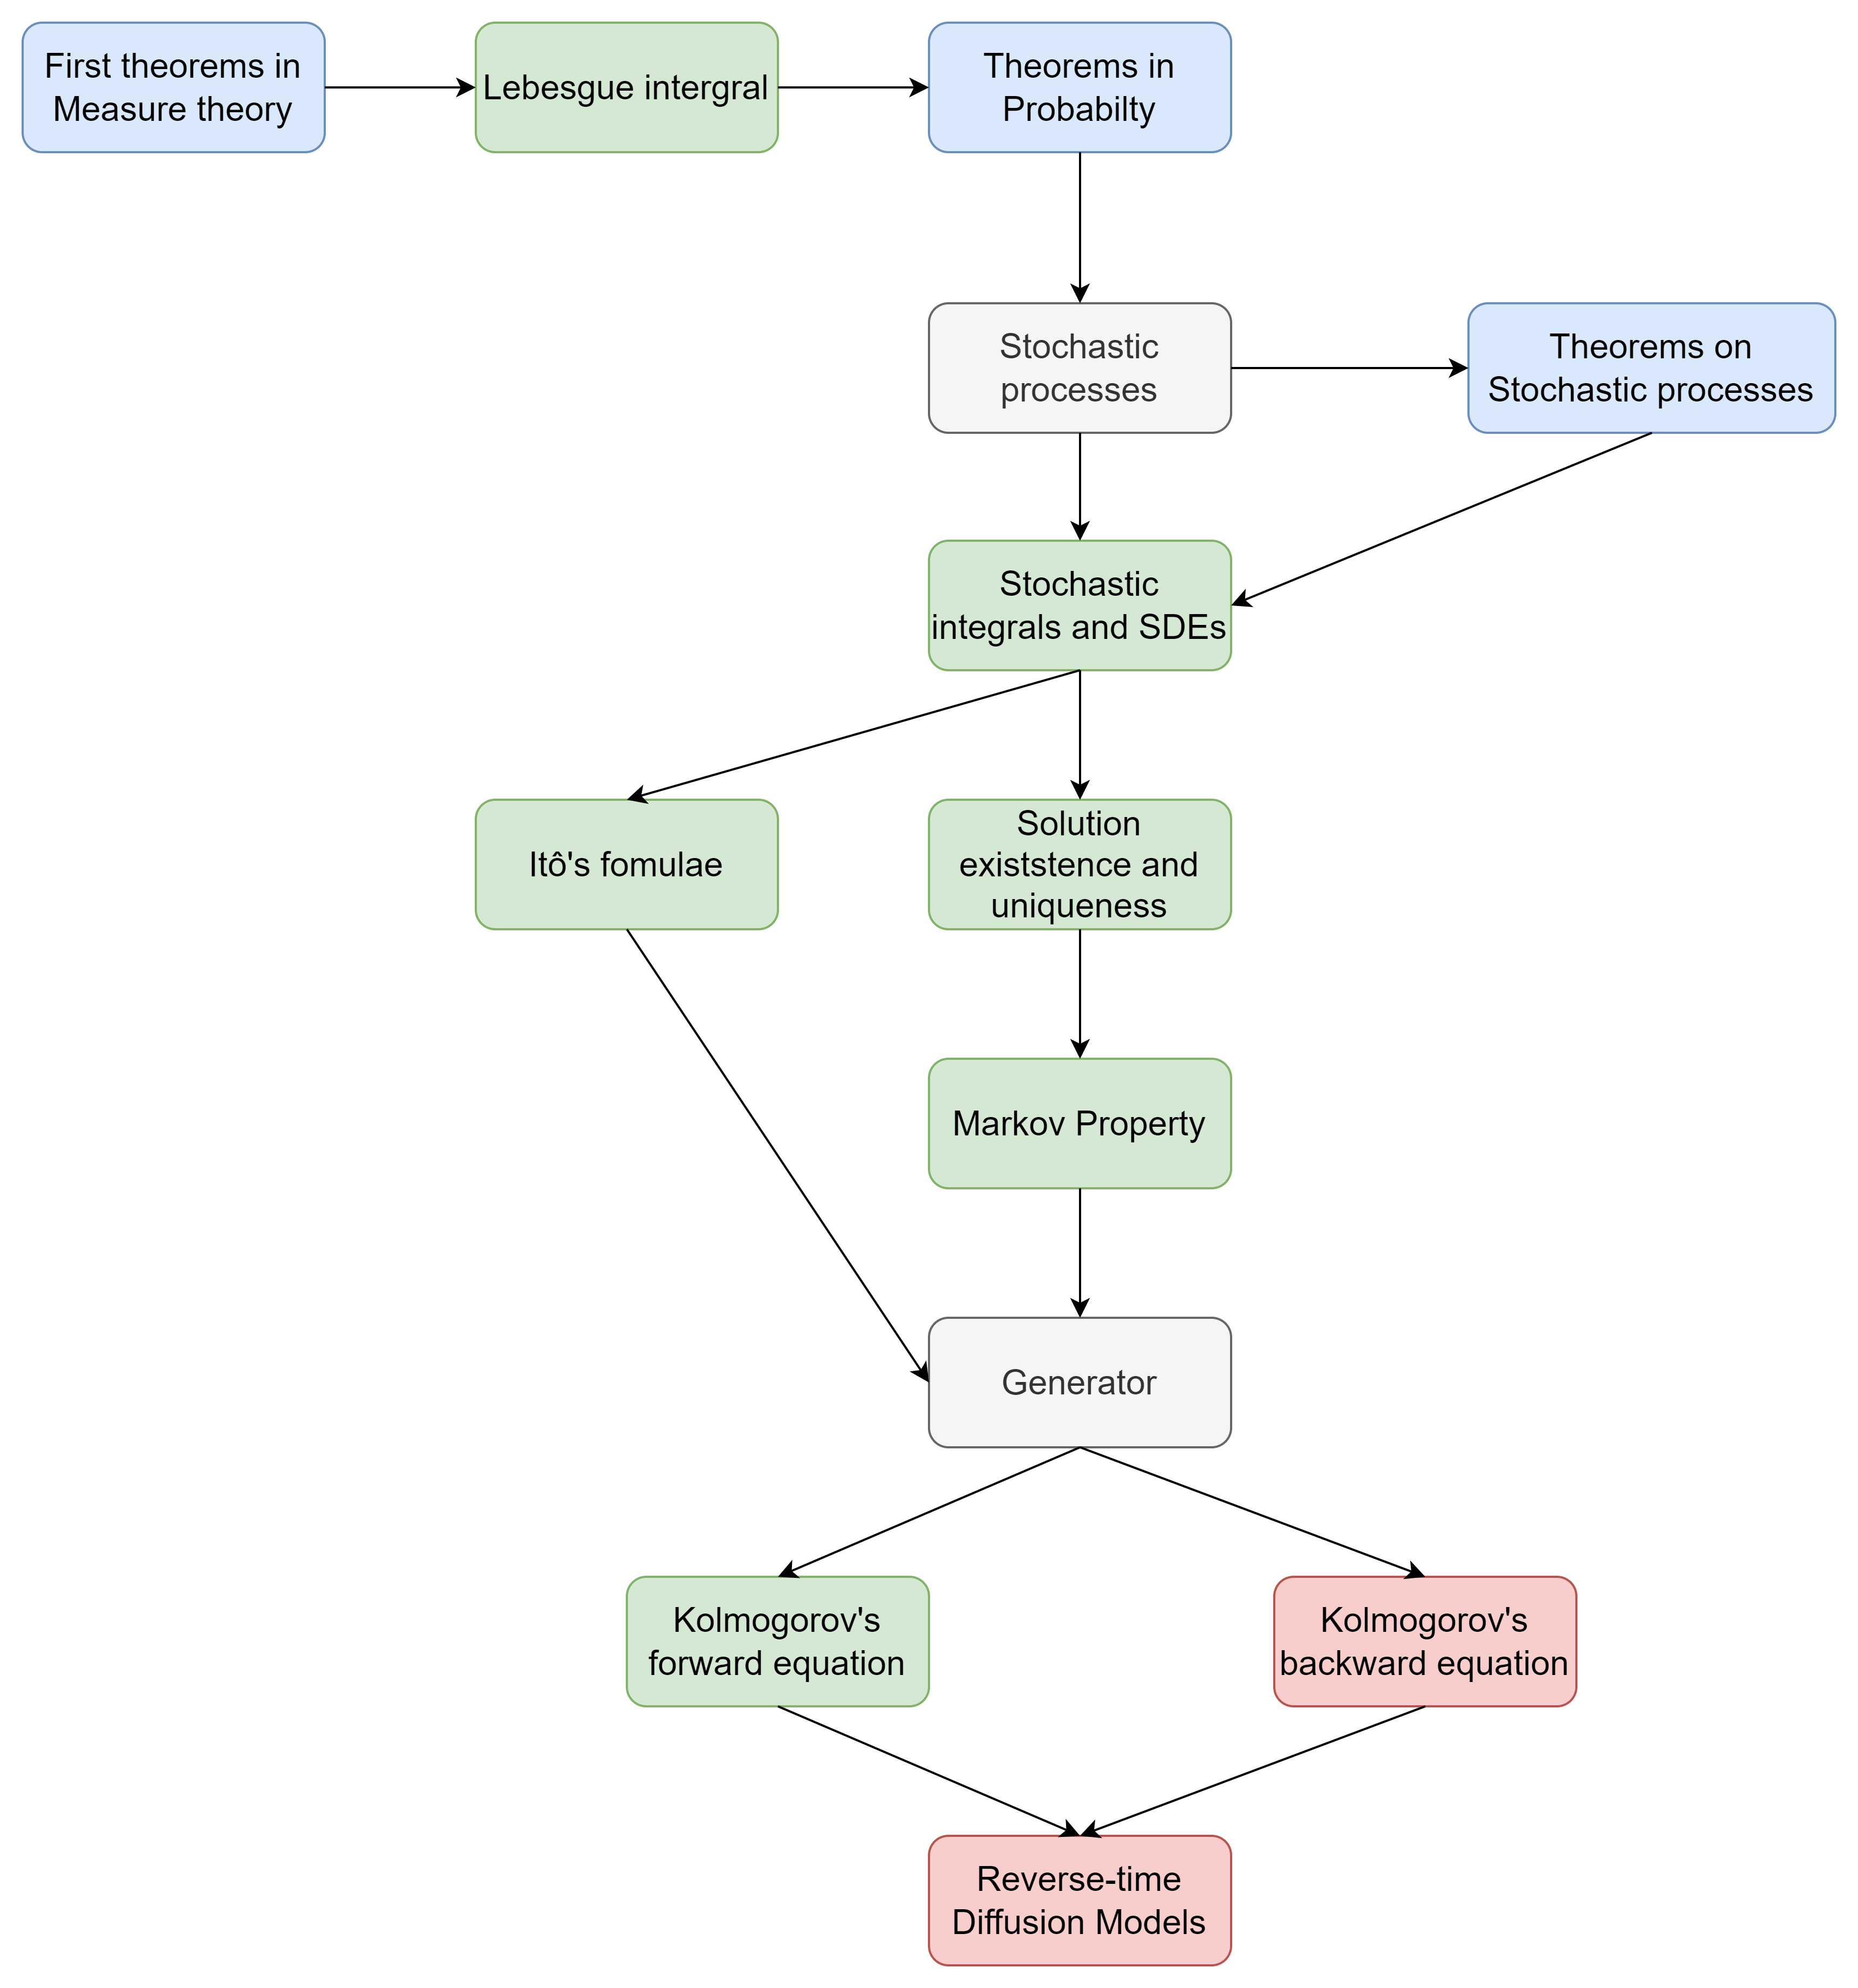
\includegraphics[width=0.75\linewidth]{img/theorem-dependency.png}
%     \vspace{0.5cm}
%     \caption{Theoretical Concept Dependency}

%     \label{figure:dep}
% \end{figure}

% In the next semester, we aim to improve the understandings by
% \begin{enumerate}
%     \item Go through all the concepts once again.
%     \item Complete the last concept related to Kolmogorov's backward equation, moving from intuition to a meticulous analysis using pure logic and complete the whole background chapter.
%     \item Explore and implement an identifier using both approaches: object detection and image segmentation, for locating watermarks in images.
%     \item Conduct additional experiments to evaluate the watermark removal pipeline. Subsequently, enhance the pipeline's performance by delving deeper into diffusion-based models after gaining a comprehensive understanding of all relevant theoretical concepts.
% \end{enumerate}

% As for predominant models given in Chapter \ref{chapter:diffusion}. We will refer to the proofs of the authors to produce a version compatible with the last theoretical aspects.

% % \section{Empirical Study}
